\chapter{自监督学习与基础模型}

尽管取得了巨大成功,但基于神经网络的监督学习通常依赖于大规模的标注数据集,收集成本很高。最近,随着一系列模型(例如,BERT [\cite{devlin2019bert}] 和 GPT-3 [\cite{brown2020language}])的兴起,人工智能和机器学习正在经历一场范式转变。这些模型在大规模广域数据上进行预训练,并且适用于各种下游任务。这些模型,被 \cite{bommasani2021opportunities} 称为基础模型,通常利用海量无标注数据,因此下游任务所需的标注数据大大减少。此外,尽管基础模型基于标准的深度学习和迁移学习,但其规模带来了新的涌现能力。这些模型通常通过自监督学习方法进行(预)训练,其中监督/标注就来自输入数据的一部分。

本章将介绍基础模型的范式和相关的基本概念。

\section{预训练与适配}\label{sec:14.1}

基础模型范式包含两个阶段:预训练(或简称为训练)和适配。首先,在一个大规模无标注数据集(例如,数十亿张无标注图像)上预训练一个大型模型。\footnote{有时候预训练也包含了大规模带标注数据,例如 ImageNet 数据集。} 然后,将预训练模型适配到下游任务(例如,从扫描图像中检测癌症)。这些下游任务通常是预测任务,其标注数据有限或者甚至没有标注数据。其直觉是,预训练模型学习到能够捕捉数据内在语义结构/信息的良好\textit{表示 (representations)},而适配阶段则根据特定下游任务对模型进行定制,例如,检索与其相关的信息。例如,在一个大规模无标注图像数据上预训练的模型可能会学习到良好的通用视觉表示/特征,然后我们将这些表示适配于解决生物医学图像任务。

下面我们形式化这两个阶段。

\subsection*{预训练}

假设有一个无标注预训练数据集 $\{x^{(1)}, x^{(2)}, \dots, x^{(n)}\}$,包含 $n$ 个位于 $\mathbb{R}^d$ 中的样本。设 $\phi_\theta$ 是一个模型,由 $\theta$ 参数化,并将输入 $x$ 映射到某个 $m$ 维表示 $\phi_\theta(x)$。(人们也将 $\phi_\theta(x) \in \mathbb{R}^m$ 称为样本 $x$ 的嵌入或特征。)我们使用预训练损失 $L_{\text{pre}}(\theta)$ 对模型 $\theta$ 进行预训练,该损失通常是所有样本上损失函数的平均值:$L_{\text{pre}}(\theta) = \frac{1}{n} \sum_{i=1}^n \ell_{\text{pre}}(\theta, x^{(i)})$。这里的 $\ell_{\text{pre}}$ 是一种所谓的单一样本 $x^{(i)}$ 上的自监督损失,因为监督信息来自数据点 $x^{(i)}$ 本身,正如后面在第 14.3 节中所示。预训练损失也可以是单个样本损失的总和。我们将在第 14.2 节和第 14.3 节中讨论两种预训练损失。

我们用一些优化器(可能是 SGD 或 ADAM [\cite{kingma2014adam}])来最小化 $L_{\text{pre}}(\theta)$。将得到的预训练模型记为 $\hat{\theta}$。

\subsection*{适配}

对于下游任务,通常有一个标注数据集 $\{(x^{(1)}_{\text{task}}, y^{(1)}_{\text{task}}), \dots, (x^{(n_{\text{task}})}_{\text{task}}, y^{(n_{\text{task}})}_{\text{task}})\}$,包含 $n_{\text{task}}$ 个样本。当 $n_{\text{task}} = 0$ 时,称为零样本学习——即下游任务没有任何标注样本。当 $n_{\text{task}}$ 相对较小(例如,在 1 到 50 之间)时,称为少样本学习。较大的 $n_{\text{task}}$(数量级从数百到数万)也非常常见。

适配算法通常以下游数据集和预训练模型 $\hat{\theta}$ 作为输入,并输出解决下游任务的 $\hat{\theta}$ 的变体。下面将讨论两种流行且通用的适配方法:线性探测 (linear probe) 和微调 (finetune)。此外,还将在 \ref{sec:14.3.1} 节中介绍另外两种针对语言问题的方法。

线性探测方法在表示层之上使用一个线性头来预测下游标签。数学上,适配后的模型输出 $w^T \phi_{\hat{\theta}}(x)$,其中 $w \in \mathbb{R}^m$ 是待学习的参数,而 $\hat{\theta}$ 是固定的预训练模型。可以使用 SGD(或其他优化器)在下游任务损失上训练 $w$ 以预测任务标签:
\begin{equation}
    \min_{w \in \mathbb{R}^m} \frac{1}{n_{\text{task}}} \sum_{i=1}^{n_{\text{task}}} \ell_{\text{task}}(y^{(i)}_{\text{task}}, w^T \phi_{\hat{\theta}}(x^{(i)}_{\text{task}})) \label{eq:14.1}
\end{equation}
例如,若下游任务是回归问题,则 $\ell_{\text{task}}(y^{(i)}_{\text{task}}, w^T \phi_{\hat{\theta}}(x^{(i)}_{\text{task}})) = (y^{(i)}_{\text{task}} - w^T \phi_{\hat{\theta}}(x^{(i)}_{\text{task}}))^2$。

微调算法对下游预测模型使用类似的结构,但会进一步微调预训练模型(而不是固定它)。具体来说,预测模型是 $w^T \phi_\theta(x)$,参数为 $w$ 和 $\theta$。我们优化 $w$ 和 $\theta$ 以适配下游数据,但用预训练模型 $\hat{\theta}$ 初始化 $\theta$。线性头 $w$ 通常随机初始化。

\begin{align}
    \minimize_{w, \theta}\  &\frac{1}{n_{\text{task}}} \sum_{i=1}^{n_{\text{task}}} \ell_{\text{task}}(y^{(i)}_{\text{task}}, w^T \phi_{\theta}(x^{(i)}_{\text{task}})) \label{eq:14.2}\\
    \text{初始化} \ 
        &w \leftarrow \text{随机向量} \label{eq:14.3}\\
        &\theta \leftarrow \hat{\theta} \label{eq:14.4}
\end{align}

存在各种其他适配方法,有时是针对特定的预训练方法而专门设计的。我们将在第 \ref{sec:14.3.1} 节中讨论其中一种。

\section{计算机视觉中的预训练方法}

本节介绍两种计算机视觉中具体的预训练方法:监督预训练和对比学习。

\subsection*{监督预训练}

在这里,预训练数据集是一个大规模\textit{标注 (labeled)} 数据集(例如,ImageNet),而预训练模型是一个使用普通监督学习训练的神经网络(去掉了最后一层)。具体来说,假设将学习到的神经网络表示为 $U \phi_{\hat{\theta}}(x)$,其中 $U$ 是最后一层(全连接层)的参数,$\hat{\theta}$ 对应于所有其他层的参数,而 $\phi_{\hat{\theta}}(x)$ 是倒数第二层的激活(用作表示)。我们丢弃 $U$,并将 $\phi_{\hat{\theta}}(x)$ 作为预训练模型。

\subsection*{对比学习}

对比学习是一种仅使用无标注数据的自监督预训练方法。其主要直觉是,一个好的表示函数 $\phi_\theta(\cdot)$ 应该将语义相似的图像映射到相似的表示,而随机的图像对通常应该具有不同的表示。例如,我们可能希望将两只哈士奇的图像映射到相似的表示,而将哈士奇和大象的图像映射到不同的表示。一种相似性的定义是同一类别的图像是相似的。使用这个定义将产生所谓的监督对比学习算法,这些算法在有标注的预训练数据集上表现良好。

在没有标注数据的情况下,可以使用数据增强来生成一对“相似”的增强图像,给定原始图像 $x$。数据增强通常意味着对原始图像 $x$ 应用\textit{随机 (random)} 裁剪、翻转和/或颜色变换来生成变体。可以对同一原始图像 $x$ 进行两次随机增强,分别记为 $\hat{x}$ 和 $\tilde{x}$,并将它们称为正样本对。可以观察到正样本对的图像通常在语义上相关,因为它们是同一图像的增强。我们将设计一个损失函数,使得 $\theta$ 能够使正样本对的表示 $\phi_\theta(\hat{x}), \phi_\theta(\tilde{x})$ 尽可能接近。

另一方面,还可以从预训练数据集中获取另一个随机图像 $z$,并从 $z$ 生成一个增强 $\hat{z}$。注意,$(\hat{x}, \hat{z})$ 来自不同的图像;因此,很有可能它们在语义上不相关。$(\hat{x}, \hat{z})$ 被称为负样本对或随机样本对。\footnote{随机样本对可能更准确,因为 $x$ 和 $z$ 仍然有可能(尽管概率很低)在语义上相关,$\hat{x}$ 和 $\hat{z}$ 也是如此。但在文献中,负样本对这个术语也很常见。} 我们将设计一个损失来推开随机样本对的表示 $\phi_\theta(\hat{x}), \phi_\theta(\hat{z})$。

有许多基于对比学习原理的最新算法,这里以 SIMCLR [\cite{chen2020simple}] 为例。损失函数定义在大小为 $B$ 的一批样本 $(x^{(1)}, \dots, x^{(B)})$ 上。算法对批次中的每个样本 $x^{(i)}$ 施加两个随机增强,分别记为 $\hat{x}^{(i)}$ 和 $\tilde{x}^{(i)}$。这样就得到大小为 $2B$ 的增广批次:$\hat{x}^{(1)}, \dots, \hat{x}^{(B)}, \tilde{x}^{(1)}, \dots, \tilde{x}^{(B)}$。SIMCLR 损失定义为\footnote{这是原始损失的一个变体和简化,它不改变本质(但可能会稍微改变效率)。
}
\[
    L_{\text{pre}}(\theta) = - \sum_{i=1}^B \log \frac{\exp(\phi_\theta(\hat{x}^{(i)})^T \phi_\theta(\tilde{x}^{(i)}))}{\exp(\phi_\theta(\hat{x}^{(i)})^T \phi_\theta(\tilde{x}^{(i)})) + \sum_{j \neq i} \exp(\phi_\theta(\hat{x}^{(i)})^T \phi_\theta(\tilde{x}^{(j)}))}.
\]
这里的直觉是,损失随着 $\phi_\theta(\hat{x}^{(i)})^T \phi_\theta(\tilde{x}^{(j)})$ 增加而增加,因此最小化损失会鼓励 $\phi_\theta(\hat{x}^{(i)})^T \phi_\theta(\tilde{x}^{(j)})$ 变小,从而使 $\phi_\theta(\hat{x}^{(i)})$ 远离 $\phi_\theta(\tilde{x}^{(j)})$。另一方面,损失随着 $\phi_\theta(\hat{x}^{(i)})^T \phi_\theta(\tilde{x}^{(i)})$ 增加而减少,因此最小化损失会鼓励 $\phi_\theta(\hat{x}^{(i)})$ 和 $\phi_\theta(\tilde{x}^{(i)})$ 变得接近。\footnote{为了理解这一点,可以验证函数 $-\log \frac{p}{p+q}$ 在 $p$ 增大时减小,而在 $q$ 增大时增大,前提是 $p, q > 0$。}


\section{预训练的大语言模型}

自然语言处理是预训练模型特别成功的另一个领域。在语言问题中,一个例子通常对应于一个文档或通常是一个词序列/片段,\footnote{在实际实现中,通常将所有数据按某种顺序串联成一个单一序列,每个样本通常对应于一个连续词的子序列,该子序列可能对应于文档的一部分或跨越多个文档。} 表示为 $x = (x_1, \dots, x_T)$,其中 $T$ 是文档/序列的长度,$x_i \in \{1, 2, \dots, V\}$ 是文档中的词,$V$ 是词汇表大小$^{6}$。\footnote{从技术上讲,词可以分解为 token,可以是词或子词(字母组合),但这里略去这一技术细节。事实上,大多数常见词本身就是一个 token。}

语言模型是一个概率模型,表示文档的概率,记为 $p(x_1, \dots, x_T)$。这个概率分布非常复杂,因为它的支撑集大小是 $V^T$——关于文档长度呈指数级增长。与其直接建模文档的分布,不如应用条件概率的链式法则将其分解如下:
\begin{equation} 
    p(x_1, \dots, x_T) = p(x_1)p(x_2|x_1)\cdots p(x_T|x_1, \dots, x_{T-1}).\label{eq:14.5}
\end{equation}
现在,每个条件概率 $p(x_t|x_1, \dots, x_{t-1})$ 的支撑集大小都是 $V$。

将条件概率 $p(x_t|x_1, \dots, x_{t-1})$ 建模为 $x_1, \dots, x_{t-1}$ 的函数,并用 $\theta$ 参数化。

参数化模型接受数值输入,因此先引入词的嵌入或表示。设 $e_i \in \mathbb{R}^d$ 是词 $i \in \{1, 2, \dots, V\}$ 的嵌入。$[e_1, \dots, e_V] \in \mathbb{R}^{d \times V}$ 被称为嵌入矩阵。

最常用的模型是 Transformer [\cite{vaswani2017attention}]。本节将介绍 Transformer 的输入输出接口,但将 Transformer 中的中间计算视为黑箱。有关更多详细信息,请参阅 Transformer 论文或更高级的课程。如图 \ref{fig:14.1} 所示,给定一个文档 $(x_1, \dots, x_T)$,首先将离散变量序列转换为相应的词嵌入 $(e_{x_1}, \dots, e_{x_T})$。并且词汇表中引入一个固定的特殊标记 $x_0 = \perp$,其对应的嵌入 $e_{x_0}$ 用于标记文档的开始。然后,将词嵌入输入到 Transformer 模型中,该模型接收一个向量序列 $(e_{x_0}, e_{x_1}, \dots, e_{x_T})$,并输出一个向量序列 $(u_1, u_2, \dots, u_{T+1})$,其中 $u_t \in \mathbb{R}^V$ 将被解释为下一个词概率分布的 logits。这里使用 Transformer 的自回归版本,其设计确保 $u_t$ 仅依赖于 $x_1, \dots, x_{t-1}$(注意,在掩码语言模型 [\cite{devlin2019bert}] 中,损失函数也不同,这一点不成立)。在本节中,我们将从 $x$ 到 $u$ 的整个映射视为一个黑箱,并将其称为 Transformer,记为 $f_\theta$,其中 $\theta$ 包括 Transformer 中的参数和输入嵌入。记 $u_t = f_\theta(x_0, x_1, \dots, x_{t-1})$,其中 $f_\theta$ 表示从输入到输出的映射。

\begin{figure}
    \centering
    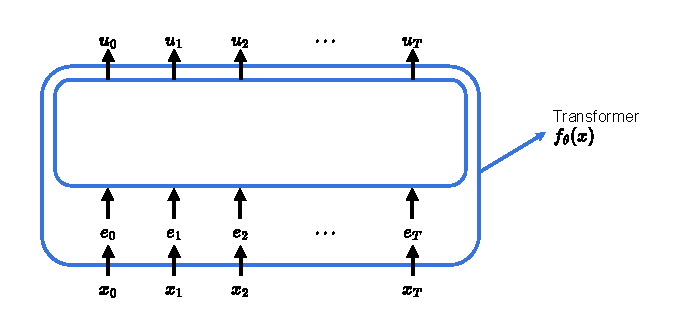
\includegraphics[width=0.7\textwidth]{figs/transformer.pdf}
    \caption{Transformer 模型的输入输出。}
    \label{fig:14.1}
\end{figure}

条件概率 $p(x_t|x_1, \dots, x_{t-1})$ 是 logits 的 softmax:
\begin{align}
    \begin{bmatrix}
        p(x_t = 1|x_1 \dots, x_{t-1})\\
        p(x_t = 2|x_1 \dots, x_{t-1})\\
        \vdots\\
        p(x_t = V|x_1 \dots, x_{t-1})
    \end{bmatrix} 
    &= \text{softmax}(u_t) \in \mathbb{R}^V \label{eq:14.6} \\
    &= \text{softmax}(f_\theta(x_0, \dots, x_{t-1})) \label{eq:14.7}
\end{align}
通过最小化在由 $\theta$ 定义的概率模型下看到数据的负对数似然,从而训练 Transformer 参数 $\theta$。这等价于最小化 logits 上的交叉熵损失。
\begin{align}
    \text{loss}(\theta) &= \frac{1}{T} \sum_{t=1}^T -\log(p_\theta(x_t|x_1, \dots, x_{t-1})) \label{eq:14.8} \\
    &= \frac{1}{T} \sum_{t=1}^T \ell_{\text{ce}}(f_\theta(x_0, x_1, \dots, x_{t-1}), x_t) \nonumber\\
    &= \frac{1}{T} \sum_{t=1}^T -\log(\text{softmax}(f_\theta(x_0, x_1, \dots, x_{t-1})))_{x_t}.\nonumber
\end{align}

\subsection*{自回归文本解码 / 生成}

给定一个自回归 Transformer,可以直接从中按顺序采样文本。给定前缀 $x_1, \dots, x_t$,利用条件分布按顺序生成文本补全 $x_{t+1}, \dots, x_T$:
\begin{align}
    x_{t+1} &\sim \text{softmax}(f_\theta(x_0, x_1, \dots, x_t)) \label{eq:14.9} \\
    x_{t+2} &\sim \text{softmax}(f_\theta(x_0, x_1, \dots, x_{t+1})) \label{eq:14.10} \\
    &\dots \label{eq:14.11} \\
    x_T &\sim \text{softmax}(f_\theta(x_0, x_1, \dots, x_{T-1})). \label{eq:14.12}
\end{align}
注意,生成的每一个 token 都被用作生成后续 token 时模型的输入。在实践中,为了进一步调整生成分布的熵/尖锐度,通常会引入一个名为 \textit{温度 (temperature)} 的参数 $\tau > 0$。当 $\tau = 1$ 时,文本从模型定义的原始条件概率中采样。随着 $\tau$ 的减小,生成的文本逐渐变得更加“确定性”。当 $\tau \to 0$ 时,这退化为贪婪解码,即从条件概率中生成概率最高的下一个 token。

\subsection{零样本学习与语境学习}\label{sec:14.3.1}

对于语言模型,有多种方法可以将预训练模型适配到下游任务。本小节将讨论其中的三种:微调、零样本学习和上下文学习。

\textbf{微调 (Finetuning)}对于自回归语言模型并不常见,但在其他变体(如掩码语言模型)中更为常见,这些变体具有类似的输入-输出接口,但预训练方式不同 [\cite{devlin2019bert}]。微调方法与第 \ref{sec:14.1} 节中介绍的通用方法相同——唯一的问题是如何定义预测任务并添加一个额外的线性头部。一种选择是将 $c_{T+1} = \phi_\theta(x_1, \dots, x_T)$ 视为表示,并使用 $w^T c_{T+1} = w^T \phi_\theta(x_1, \dots, x_T)$ 来预测任务标签。如第 \ref{sec:14.1} 节所述,将 $\theta$ 初始化为预训练模型 $\hat{\theta}$,然后同时优化 $w$ 和 $\theta$。

\textbf{零样本 (Zero-shot)} 适配或零样本学习是指下游任务没有输入-输出对的情景。对于语言问题任务,通常将任务格式化为问题或通过自然语言的完形填空形式。例如:
\[
    x_{\text{task}} = (x_{\text{task},1}, \dots, x_{\text{task},T}) = \text{“光速是常数吗?”}
\]
然后,计算此问题下,语言模型所预测的最有可能的下一个词,即计算下式 $\text{argmax}_{x_{T+1}} p(x_{T+1} | x_{\text{task},1}, \dots, x_{\text{task},T})$。在这种情况下,如果最有可能的下一个词 $x_{T+1}$ 是“否”,则任务完成。(光速仅在真空中是常数。)注意,有许多方法可以从语言模型中解码答案,例如,除了计算 argmax,也可以使用语言模型直接生成几个词作为答案。寻找利用语言模型的最佳方法是一个活跃的研究问题。

\textbf{语境学习 (In-context learning)} 主要用于少样本情景,此时我们有少量带标签的例子 $(x_{\text{task}}^{(1)}, y_{\text{task}}^{(1)}), \dots, (x_{\text{task}}^{(n_{\text{task}})}, y_{\text{task}}^{(n_{\text{task}})})$。给定一个测试例子 $x_{\text{test}}$,通过以某种格式将带标签的例子和测试例子连接起来,构建一个文档 $(x_1, \dots, x_T)$,这在上下文中通常称为“提示 (prompt)”。例如,可以按如下方式构建提示:
\begin{align*}
    x_1, \cdots, x_T \enspace = \enspace “
        &\text{Q: 2 $\sim$ 3 = ?} \quad & \textcolor{red}{x^{(1)}_\text{task}}\\
        &\text{A: 5} \quad & \textcolor{red}{y^{(1)}_\text{task}}\\
        &\text{Q: 6 $\sim$ 7 = ?} \quad & \textcolor{red}{x^{(2)}_\text{task}}\\
        &\text{A: 13} \quad & \textcolor{red}{y^{(2)}_\text{task}}\\
        &\cdots \\
        &\text{Q: 15 $\sim$ 2 = ?}” \quad & \textcolor{red}{x_{\text{test}}}
\end{align*}

然后,让预训练模型生成最有可能的 $x_{T+1}, x_{T+2}, \dots$。在这种情况下,如果模型能从少量例子中“学会”符号 $\sim$ 代表加法,将得到以下结果,表明答案是 17。
\[
    x_{T+1}, x_{T+2}, \dots = \text{“A: 17”}.
\]
基础模型领域是一个非常新且快速发展的领域。这里仅试图在概念层面介绍这些模型,并进行了大量简化。关于更多细节,请参阅其他材料,例如 \cite{bommasani2021opportunities}。